\documentclass[conference]{IEEEtran}
\IEEEoverridecommandlockouts
\usepackage{cite}
\usepackage{amsmath,amssymb,amsfonts}
\usepackage{algorithmic}
\usepackage{graphicx}
\usepackage{textcomp}
\usepackage{xcolor}
\usepackage{booktabs}
\usepackage{multirow}
\usepackage{tikz}
\usetikzlibrary{arrows.meta,positioning,shapes.geometric,fit}
\usepackage{url}
\def\BibTeX{{\rm B\kern-.05em{\sc i\kern-.025em b}\kern-.08em T\kern-.1em\lower.7ex\hbox{E}\kern-.125em X}}

\begin{document}

\title{When to Label? Annotation-Budget-Aware Selection among Zero-Shot, Pseudo-Label, and Fine-Tuned Object Detectors}

\author{\IEEEauthorblockN{[Author Name(s) -- to be filled in]}
\IEEEauthorblockA{\textit{[Affiliation]}\\
{[email]}}}

\maketitle
\begin{abstract}
Choosing how to spend an annotation budget when deploying an object detector is hard: an open-vocabulary detector can be used zero-shot, used as a teacher whose pseudo-labels train a small student, or replaced by a detector fine-tuned on manual labels. We present a budget-controlled comparison of these strategies on two public domains, HomeObjects-3K (common household nouns) and Construction-PPE (domain-specific classes, including absence of equipment), with nested labeled subsets of 0--400 images, matched training compute and a single evaluator. The best strategy depends on the domain: on HomeObjects, zero-shot YOLOE-11s (55.3 mAP$_{50}$) was not surpassed by any trained YOLO11n student up to 400 labels (28.4), although a compute ablation shows the gap narrows from 27 to about 14 points with more training; on Construction-PPE, zero-shot reaches only 23.6 and fine-tuning on 10 labeled images already exceeds it (27.4), reaching 41.1 at 400. Pseudo-label distillation at best matched the teacher, and mixing noisy pseudo-labels with 200 gold labels lowered accuracy by 9.7 points compared with using the gold labels alone. We further propose a calibration of the pseudo-label threshold on the labeled images (no measurable effect here), a learning-curve-based strategy selector (correct in all 12 low-difficulty test cases, which contain no real crossover), and quantify that 50 labeled images estimate zero-shot mAP$_{50}$ to within about 2.5--3.4 points. Results are small-scale (two datasets, two seeds, CPU-limited students) and should be validated with stronger teachers and larger budgets.
\end{abstract}

\begin{IEEEkeywords}
open-vocabulary object detection, annotation budget, pseudo-labeling, teacher--student learning, fine-tuning, strategy selection
\end{IEEEkeywords}
\section{Introduction}
Deploying an object detector in a new domain forces a practitioner to choose \emph{how} to spend an annotation budget. Three families of strategies are now realistic. (i)~An open-vocabulary detector such as YOLO-World~\cite{cheng2024yoloworld}, Grounding~DINO~\cite{liu2024groundingdino}, OWLv2~\cite{minderer2023owlv2} or YOLOE~\cite{wang2025yoloe} can be prompted with class names and used \emph{zero-shot}, at zero labeling cost. (ii)~Such a detector can act as a \emph{teacher} that pseudo-labels an unlabeled image pool, from which a small, fast \emph{student} (e.g., YOLO) is trained~\cite{son2024teacherstudent,xin2024dart}. (iii)~A pretrained closed-set detector can be \emph{fine-tuned} on manually labeled images. Which of these is best depends on the number of labeled images that can be afforded, on how far the target label space is from what the open-vocabulary detector has seen, and on the deployment constraints on latency.

The literature mostly improves one strategy at a time: stronger open-vocabulary architectures~\cite{cheng2024yoloworld,liu2024groundingdino,minderer2023owlv2,wang2025yoloe}, better pseudo-labeling~\cite{gao2022pseudobox,liu2021unbiased,xu2021softteacher}, or few-shot fine-tuning recipes~\cite{wang2020tfa}. Recent benchmarks show that zero-shot detectors can fail badly on concepts that are rare in pre-training data~\cite{robicheaux2025rf100vl}, and that pseudo-labels alone can rival supervised training in some domains~\cite{abid2025waste}. What is missing is a \emph{budget-indexed} comparison: given $N$ labeled images, which strategy should be used, how reliable is that decision, and can it be made \emph{before} the labeling money is spent?

This paper makes four contributions.
\begin{itemize}
\item \textbf{Budget-controlled benchmark.} We compare zero-shot detection, teacher--student pseudo-labeling, and fine-tuning under identical evaluation, nested labeled subsets ($N\in\{0,10,\dots,400\}$ images), matched training compute, and multiple seeds, on two domains that differ in how well the zero-shot teacher fits them, and report the budgets at which the ranking of strategies changes.
\item \textbf{Gold-calibrated pseudo-labeling (TS-cal).} We use the same $N$ labeled images that fine-tuning would consume to select the teacher's pseudo-label confidence threshold, so that labeled data serve both as supervision and as a calibration set for the teacher.
\item \textbf{Cost-aware strategy selector.} We fit per-strategy learning curves on small pilot budgets and extrapolate to choose a strategy for a larger budget, and we evaluate the choices against measured outcomes (regret relative to an oracle and to fixed rules).
\item \textbf{Pilot-set reliability.} We quantify how many labeled images are needed merely to \emph{measure} the zero-shot detector's accuracy and to order it against a fine-tuned model, a prerequisite for any budget-aware decision.
\end{itemize}
All code, raw per-image statistics, and scripts are released with the paper.

\section{Related Work}
\textbf{Open-vocabulary detection.} GLIP~\cite{li2022glip} casts detection as phrase grounding; OWL-ViT/OWLv2~\cite{minderer2022owlvit,minderer2023owlv2}, ViLD~\cite{gu2022vild} and Detic~\cite{zhou2022detic} transfer image-level vision--language knowledge (e.g., CLIP~\cite{radford2021clip}) to box prediction; Grounding~DINO~\cite{liu2024groundingdino} fuses language early in a DETR-style detector. YOLO-World~\cite{cheng2024yoloworld} and YOLOE~\cite{wang2025yoloe} bring open-vocabulary prompting to the real-time YOLO family. Our zero-shot detector is YOLOE with the MobileCLIP~\cite{vasu2024mobileclip} text encoder. One-shot retail detectors such as SiamYOLOv8~\cite{desmarescaux2025siamyolov8} target accuracy with a single reference image rather than the choice between strategies.

\textbf{Pseudo-labeling and teacher--student detection.} Semi-supervised detectors such as Unbiased Teacher~\cite{liu2021unbiased} and Soft Teacher~\cite{xu2021softteacher} bootstrap from a labeled subset. With vision--language teachers, Gao \emph{et al.}~\cite{gao2022pseudobox} generate pseudo boxes for open-vocabulary training; Son and Jung~\cite{son2024teacherstudent} train YOLO on Grounding~DINO labels and report no clear degradation relative to manual labels; DART~\cite{xin2024dart} automates a diversification--annotation--review--training pipeline; and Abid \emph{et al.}~\cite{abid2025waste} show that pseudo-labels from vision--language models can improve YOLO on waste detection. These works study one pipeline at fixed supervision; none varies the manual-label budget to locate where each strategy wins.

\textbf{Benchmarks of zero-shot versus few-shot detection.} Roboflow100-VL~\cite{robicheaux2025rf100vl} evaluates vision--language detectors on 100 diverse datasets in zero-, few-shot, semi-supervised and fully supervised regimes and shows large zero-shot failures outside common concepts. Our study is narrower but complementary: it sweeps the labeling budget densely within a domain, controls training compute, and turns the measurements into a selection rule.

\textbf{Annotation cost and learning curves.} Box annotation is costly: on the order of seconds per box even with efficient protocols~\cite{su2012crowdsourcing,papadopoulos2017extreme}. Active learning for detection~\cite{brust2018active} decides \emph{which} images to label; we address the complementary question of \emph{which learning strategy} to buy with a given number of labels. Our selector relies on the empirical regularity of learning curves~\cite{cortes1993curves,hestness2017scaling}.
\section{Problem Formulation and Method}
\subsection{Setting}
Let $\mathcal{U}$ be a pool of unlabeled images from the target domain, $\mathcal{C}$ a known set of $K$ class names, and $N\ge 0$ the number of images that can be fully annotated (all boxes, all classes). The labeled set $\mathcal{L}_N\subset\mathcal{U}$ is nested across budgets, $\mathcal{L}_{N}\subset\mathcal{L}_{N'}$ for $N<N'$. A \emph{strategy} $s$ maps $(\mathcal{U},\mathcal{L}_N,\mathcal{C})$ to a detector, and we measure its accuracy $a_s(N)$ as mAP on a held-out set, together with its annotation cost $c_{\text{ann}}(N)$ and compute cost.

\subsection{Candidate strategies}
\textbf{ZS (zero-shot).} An open-vocabulary detector $T$ (the \emph{teacher}) is prompted with one fixed text phrase per class. It needs no labels, so $a_{\text{ZS}}(N)$ is constant in $N$, and its test-time cost is that of $T$.

\textbf{FT (fine-tuning).} A COCO-pretrained closed-set detector $S$ (the \emph{student}) is fine-tuned on $\mathcal{L}_N$ only (undefined for $N=0$).

\textbf{TS (teacher--student).} $T$ labels every image in $\mathcal{U}\setminus\mathcal{L}_N$; detections with confidence $\ge\tau$ become pseudo-boxes, and $S$ is trained on $\mathcal{L}_N$ (gold) $\cup\ (\mathcal{U}\setminus\mathcal{L}_N)$ (pseudo). With $N=0$ this is pure distillation of the zero-shot teacher into a faster student, with no manual labels.

\textbf{TS-cal (proposed).} Identical to TS except that $\tau$ is chosen from a small grid $\mathcal{T}$ to maximize micro-$F_1$ at IoU~0.5 of the \emph{teacher's} predictions on $\mathcal{L}_N$:
\begin{equation}
\tau^\star(N)=\arg\max_{\tau\in\mathcal{T}} F_1\big(T_{\ge\tau};\mathcal{L}_N\big),
\end{equation}
falling back to the default $\tau_0$ when $N=0$. This costs no extra annotation and no extra training: the labeled images that fine-tuning would consume are reused as a calibration set for the teacher.

\subsection{Cost model}
Annotation time for $N$ images is modeled as
\begin{equation}
c_{\text{ann}}(N)=N\,(t_{\text{img}}+\bar b\,t_{\text{box}}),
\end{equation}
where $\bar b$ is the mean number of boxes per image in the domain (measured), $t_{\text{img}}=5$\,s of viewing time and $t_{\text{box}}$ the per-box drawing time. Because per-box times in the literature range from several seconds~\cite{papadopoulos2017extreme} to tens of seconds~\cite{su2012crowdsourcing}, we treat $t_{\text{box}}\in\{5,10,35\}$\,s as a sensitivity range rather than a measurement. Pseudo-labels are assumed to cost no human time.

\subsection{Learning-curve strategy selector}
For each learned strategy $s\in\{\text{TS},\text{TS-cal},\text{FT}\}$ the practitioner observes accuracy at a few small pilot budgets $N_1<\dots<N_m$ (cheap, because small $N$ means small training sets). We fit
\begin{equation}
\text{loglin: } a_s(N)=\alpha_s+\beta_s\ln N,\qquad
\text{power: } a_s(N)=\alpha_s-\beta_s N^{-\gamma_s},
\end{equation}
and extrapolate to the target budget $N$. The zero-shot accuracy is a constant measured on the labeled pilot set. The selector recommends
\begin{equation}
\hat s(N)=\arg\max_{s}\ \hat a_s(N)-\lambda\, h_s(N),
\end{equation}
where $h_s$ is a cost in hours and $\lambda\ge0$ trades accuracy against cost ($\lambda=0$ in our evaluation, which isolates the accuracy prediction). Section~\ref{sec:selector} measures how often $\hat s(N)$ matches the strategy that is best in hindsight and how much accuracy is lost when it does not (\emph{regret}).

\begin{figure}[t]
\centering
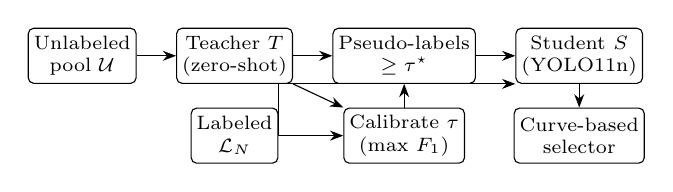
\begin{tikzpicture}[node distance=3mm and 5mm, every node/.style={font=\scriptsize}, box/.style={draw,rounded corners=2pt,align=center,inner sep=2pt,minimum height=7mm}]
\node[box] (u) {Unlabeled\\pool $\mathcal{U}$};
\node[box,right=of u] (t) {Teacher $T$\\(zero-shot)};
\node[box,right=of t] (p) {Pseudo-labels\\$\ge\tau^\star$};
\node[box,right=of p] (s) {Student $S$\\(YOLO11n)};
\node[box,below=of t] (l) {Labeled\\$\mathcal{L}_N$};
\node[box,below=of p] (c) {Calibrate $\tau$\\(max $F_1$)};
\node[box,below=of s] (sel) {Curve-based\\selector};
\draw[-{Stealth}] (u)--(t); \draw[-{Stealth}] (t)--(p); \draw[-{Stealth}] (p)--(s);
\draw[-{Stealth}] (l)--(c); \draw[-{Stealth}] (t.south east)--(c.north west); \draw[-{Stealth}] (c)--(p);
\draw[-{Stealth}] (l.east)--++(0,0)|-(s.south west);
\draw[-{Stealth}] (s)--(sel);
\end{tikzpicture}
\caption{Overview. Labeled images supervise the student directly (FT/TS) and calibrate the teacher's pseudo-label threshold (TS-cal); accuracy at small pilot budgets feeds the selector.}
\label{fig:overview}
\end{figure}

\section{Experimental Setup}
\textbf{Datasets.} We use two public detection datasets distributed with the Ultralytics package~\cite{ultralyticsdatasets}, chosen because they differ in how closely their label spaces match natural-language object names. \emph{HomeObjects-3K}: 12 household categories (bed, sofa, chair, \dots), 2\,285 training and 404 validation images. \emph{Construction-PPE}: 11 categories including both equipment (helmet, vest, \dots) and absence classes (no\_helmet, no\_goggle, \dots) that are hard to express as a noun phrase; 1\,132 training, 143 validation and 141 test images. We evaluate on the validation split (HomeObjects) and validation+test (PPE, 284 images). The retail checkout dataset RPC~\cite{wei2019rpc} originally planned for this project was not accessible in our offline-restricted environment, so we do not report retail results.

\textbf{Models.} Teacher/zero-shot: YOLOE-11s~\cite{wang2025yoloe} with MobileCLIP text prompts, inference at $640$\,px. Student/fine-tuned: YOLO11n~\cite{jocher2024yolo11} initialised from COCO~\cite{lin2014coco} weights, trained and tested at $320$\,px. The text prompt per class was fixed before running any experiment (Table~\ref{tab:prompts}) and never tuned. Grounding~DINO and OWLv2 weights were not accessible to us; replacing the teacher with them is a drop-in change (\texttt{src/aovd/detectors.py}).

\textbf{Budgets and seeds.} For every seed we draw a random unlabeled pool of $400$ training images and take the first $N\in\{10,25,50,100,200,400\}$ images of a seeded permutation as the labeled subset (nested). TS and TS-cal use the whole pool (gold labels for $\mathcal{L}_N$, teacher pseudo-labels for the rest); FT uses $\mathcal{L}_N$ only. Thresholds: $\tau_0=0.25$, $\mathcal{T}=\{0.10,0.25,0.40\}$.

\textbf{Training protocol.} Every student run gets the same compute: 4\,800 image visits (e.g., 480 epochs for $N{=}10$ and 12 epochs for $N{=}400$), AdamW selected by the Ultralytics `auto' rule, batch 16, default augmentations, on CPU (4 cores shared by two concurrent jobs). Matching compute rather than epochs avoids favoring strategies with larger training sets.

\textbf{Metrics.} A single evaluator (COCO-style 101-point AP, IoU $0.50{:}0.95$, class-averaged, confidence threshold $0.001$, NMS IoU $0.7$) scores every method on the same images. We report mAP$_{50}$ and mAP$_{50:95}$ as mean$\pm$std over seeds.

\begin{table}[t]
\caption{Fixed zero-shot text prompts (dataset label $\rightarrow$ prompt, when different).}
\label{tab:prompts}
\centering\footnotesize
\begin{tabular}{p{0.9in}p{2.3in}}
\toprule
HomeObjects & tv$\rightarrow$``television''; all other class names used verbatim\\
Construction-PPE & helmet$\rightarrow$``hard hat''; vest$\rightarrow$``safety vest''; goggles$\rightarrow$``safety goggles''; none$\rightarrow$``person without protective equipment''; no\_helmet$\rightarrow$``head without helmet''; no\_goggle$\rightarrow$``face without goggles''; no\_gloves$\rightarrow$``bare hand''; no\_boots$\rightarrow$``bare foot''; gloves, boots, Person verbatim\\
\bottomrule
\end{tabular}
\end{table}
\section{Results}
All numbers are means over two seeds (random labeled/unlabeled pools); a third seed was started but not completed, so the standard deviations are over $n{=}2$ and are only a rough indication of variability. Zero-shot results are deterministic given the prompts.

\subsection{Accuracy versus annotation budget}
Table~\ref{tab:main} and Fig.~\ref{fig:curves} give the central result: the best strategy depends on the domain.

\textbf{Construction-PPE (weak zero-shot fit).} The zero-shot teacher reaches only 23.6 mAP$_{50}$ because half of the label space (absence classes such as no\_helmet) is not expressible as a noun phrase. Fine-tuning on just $N{=}10$ labeled images (about 14 minutes of annotation under our default cost model) already exceeds it (27.4), and accuracy rises steadily to 41.1 at $N{=}400$. Teacher--student training \emph{without} gold labels reproduces the teacher (22.3 vs.\ 23.6) and does not exceed zero-shot until the mixed pool contains mostly gold labels ($N{=}200$: 30.9; $N{=}400$ is identical to FT by construction, as the pool has no unlabeled images left). Notably, mixing noisy pseudo-labels with $N$ gold labels is \emph{worse} than discarding them: at $N{=}200$, FT on the 200 gold images alone gets 40.6 against 30.9 for TS with 200 additional pseudo-labeled images, i.e., a 9.7-point loss.

\textbf{HomeObjects-3K (strong zero-shot fit).} The label space is made of common nouns and zero-shot reaches 55.3 mAP$_{50}$. No trained student surpasses it at any budget up to $N{=}400$ (FT 28.4, TS 28.4 at $N{=}400$). FT and TS are indistinguishable from $N{\approx}50$ upward, and both are far below the teacher. Here the right decision is to label nothing and deploy the zero-shot detector, or to spend the budget elsewhere.

\begin{table}[t]
\caption{mAP$_{50}$ ($\pm$std over seeds) / mAP$_{50:95}$ (\%) versus the number of labeled images $N$. ``Ann.\ h'' is annotation time under $t_{img}{=}5$\,s, $t_{box}{=}10$\,s. TS at $N{=}0$ uses no manual labels; FT is undefined there. At $N{=}400$ the pool contains no unlabeled images, so TS$\equiv$FT.}
\label{tab:main}
\centering\scriptsize
\setlength{\tabcolsep}{2.5pt}
\begin{tabular}{rrcccc}
\toprule
$N$ & Ann.\ h & FT & TS & TS-cal & seeds\\
\midrule
\multicolumn{6}{l}{\textit{HomeObjects-3K} (zero-shot: mAP$_{50}$ 55.3, mAP$_{50:95}$ 37.0)} \\
0 & 0.00 & -- & 23.8$\pm$1.0 / 14.0 & -- & 2 \\
10 & 0.24 & 10.9$\pm$1.6 / 5.3 & 23.6$\pm$0.3 / 13.8 & 23.6$\pm$0.3 / 13.8 & 2 \\
25 & 0.61 & 18.4$\pm$1.1 / 9.7 & 24.3$\pm$0.1 / 14.5 & 24.3$\pm$0.1 / 14.5 & 2 \\
50 & 1.21 & 24.0$\pm$1.8 / 13.1 & 24.1$\pm$1.3 / 14.2 & 24.1$\pm$1.3 / 14.2 & 2 \\
100 & 2.43 & 25.3$\pm$0.4 / 14.1 & 25.0$\pm$0.4 / 14.7 & 25.0$\pm$0.4 / 14.7 & 2 \\
200 & 4.85 & 26.4$\pm$0.4 / 15.3 & 26.6$\pm$0.6 / 15.8 & 26.6$\pm$0.6 / 15.8 & 2 \\
400 & 9.71 & 28.4$\pm$0.3 / 16.7 & 28.4$\pm$0.3 / 16.7 & 28.4$\pm$0.3 / 16.7 & 2 \\
\midrule
\multicolumn{6}{l}{\textit{Construction-PPE} (zero-shot: mAP$_{50}$ 23.6, mAP$_{50:95}$ 8.4)} \\
0 & 0.00 & -- & 22.3$\pm$0.2 / 7.9 & -- & 2 \\
10 & 0.24 & 27.4$\pm$0.8 / 11.7 & 22.9$\pm$0.2 / 8.3 & 23.7$\pm$0.5 / 8.6 & 2 \\
25 & 0.59 & 31.8$\pm$0.8 / 14.1 & 23.5$\pm$0.7 / 8.4 & 23.5$\pm$0.7 / 8.4 & 2 \\
50 & 1.19 & 37.0$\pm$1.6 / 16.8 & 24.7$\pm$0.4 / 9.3 & 24.7$\pm$0.4 / 9.3 & 2 \\
100 & 2.37 & 38.8$\pm$1.0 / 17.7 & 25.9$\pm$0.5 / 10.1 & 25.9$\pm$0.5 / 10.1 & 2 \\
200 & 4.74 & 40.6$\pm$0.2 / 19.4 & 30.9$\pm$0.1 / 13.0 & 30.9$\pm$0.1 / 13.0 & 2 \\
400 & 9.49 & 41.1$\pm$0.2 / 19.4 & 41.1$\pm$0.2 / 19.4 & 41.1$\pm$0.2 / 19.4 & 2 \\
\midrule
\bottomrule
\end{tabular}
\end{table}

\begin{figure}[t]
\centering
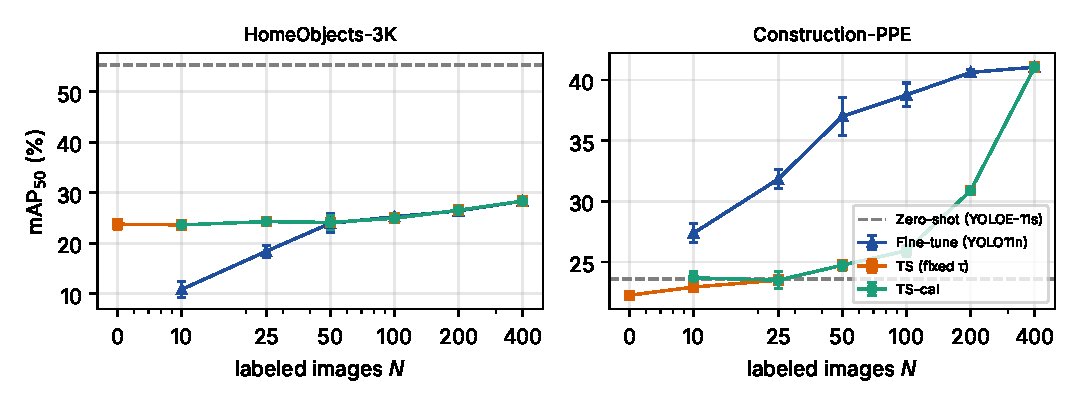
\includegraphics[width=\columnwidth]{figs/learning_curves.pdf}
\caption{mAP$_{50}$ versus labeled images (mean $\pm$ std, 2 seeds). The dashed line is the zero-shot teacher.}
\label{fig:curves}
\end{figure}

\subsection{Is the HomeObjects result a compute artifact?}
Our students are small, trained on CPU at $320$\,px for a fixed budget of 4\,800 image visits, which is likely too little for a strong detector. We therefore re-ran fine-tuning at $N{=}400$ (seed~0 only) with $4\times$ the training visits, and with input size $640$ (Table~\ref{tab:abl}). More compute helps substantially: FT improves from 28.4 to 41.5 (4$\times$ visits) or 40.7 (640\,px) on HomeObjects and from 41.1 to 48.6 on PPE. On HomeObjects the zero-shot detector (55.3) still wins at $N{=}400$, but the gap shrinks from 27 to about 14 points, so we \emph{cannot} claim that zero-shot beats fine-tuning there at convergence, only within our compute budget. We did not run the corresponding ablation for TS or for larger $N$, nor train to convergence, so the crossover for HomeObjects may lie above $N{=}400$ and the absolute numbers of all trained students are lower bounds.

\begin{table}[t]
\caption{Compute sensitivity of FT at $N{=}400$ (mAP$_{50}$ \%; ablations: seed 0 only, run alone on 4 CPU threads; main column: mean of 2 seeds; ``--'': not run).}
\label{tab:abl}
\centering\footnotesize
\begin{tabular}{lcccc}
\toprule
& Main (320\,px, $1\times$) & $4\times$ visits & 640\,px & Zero-shot\\
\midrule
HomeObjects-3K & 28.4 & 41.5 & 40.7 & 55.3 \\
Construction-PPE & 41.1 & 48.6 & -- & 23.6 \\
\bottomrule
\end{tabular}
\end{table}

\subsection{Annotation cost}
Fig.~\ref{fig:cost} plots accuracy against annotation time. On PPE, reaching 75\% of the best FT accuracy observed in our grid (30.8 mAP$_{50}$) takes $N{=}25$ labeled images for FT, about 0.6\,h at $t_{box}{=}10$\,s (0.3\,h at 5\,s, 2.0\,h at 35\,s), whereas TS reaches that level only at $N{=}200$ (4.7\,h). Zero-shot never reaches it. The ranking of strategies does not depend on $t_{box}$, because the cost model is linear in $N$ for all learned strategies; it only rescales the horizontal axis.

\begin{figure}[t]
\centering
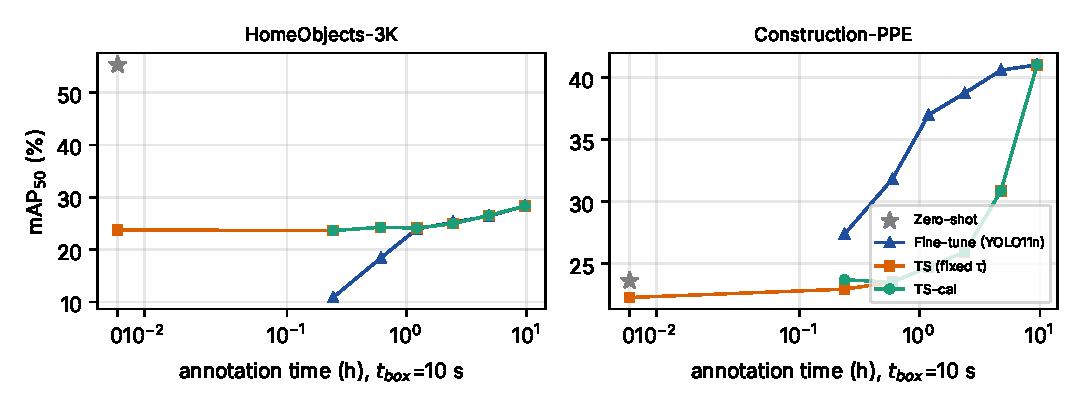
\includegraphics[width=\columnwidth]{figs/cost_accuracy.pdf}
\caption{Accuracy versus annotation time ($t_{box}{=}10$\,s). Zero-shot costs no annotation.}
\label{fig:cost}
\end{figure}

\subsection{Gold-calibrated pseudo-label threshold}
TS-cal selected the default $\tau_0{=}0.25$ in 23 of 24 (dataset, seed, $N$) cases, so for those it is identical to TS by construction. In the single case where it chose a different threshold ($\tau{=}0.10$, PPE, $N{=}10$, seed~1) mAP$_{50}$ rose by 1.5 points, which is within the seed-to-seed variation we observe. Our grid $\{0.1,0.25,0.4\}$ and the F$_1$ criterion thus provide \emph{no measurable benefit} here; the claimed contribution is a mechanism, not an effect we have demonstrated.

\subsection{Strategy selector}\label{sec:selector}
We fit each learned strategy's curve on the pilot budgets $N\in\{10,25,50\}$ of one seed and let the selector choose a strategy for $N\in\{100,200,400\}$, comparing with the strategy that was best in hindsight on the same seed (Table~\ref{tab:sel}; 12 cases: 2 datasets $\times$ 2 seeds $\times$ 3 budgets). Both curve families chose the best strategy in all 12 cases (regret 0), versus a mean regret of 8.3 mAP$_{50}$ points for always using zero-shot, 14.3 for always fine-tuning (and for the rule ``fine-tune once $N\ge100$''), and 18.1 for always using TS. We stress that this evidence is weak: the winner is the same at every budget within each dataset (zero-shot on HomeObjects, FT on PPE) and the cases are strongly correlated, so a perfect score tests extrapolation in a regime where no crossover occurs within $[100,400]$. The selector has not been tested where curves actually cross inside the extrapolation range.

\begin{table}[t]
\caption{Selector evaluated by extrapolating from $N\le50$ to $N\in\{100,200,400\}$. Hit: chosen strategy within 0.5 point of best (\%); regret in mAP$_{50}$ points (mean over 12 cases) for the selector and for fixed policies.}
\label{tab:sel}
\centering\scriptsize
\setlength{\tabcolsep}{2.5pt}
\begin{tabular}{llrrrrrrr}
\toprule
curve & strategies & cases & hit & selector & ZS & TS & FT & FT$_{N\ge100}$\\
\midrule
loglin & ZS/TS/FT & 12 & 100 & 0.00 & 8.26 & 18.11 & 14.33 & 14.33 \\
power & ZS/TS/FT & 12 & 100 & 0.00 & 8.26 & 18.11 & 14.33 & 14.33 \\
\bottomrule
\end{tabular}
\end{table}

\subsection{How many labeled images are needed to measure zero-shot accuracy?}
A budget-aware decision requires an estimate of the zero-shot detector's accuracy, which needs labeled data. Table~\ref{tab:pilot} reports the error of mAP$_{50}$ estimated on a random subset of $n$ labeled images relative to the full evaluation set (200 random subsets). The estimate is noisy and biased upward for small $n$ (subsets contain fewer classes, and rare hard classes are missing): with $n{=}10$ the mean absolute error is 7--9 points; $n{=}50$ brings it to 2.5--3.4; and $n{=}100$ to 1.4--2.6. For ordering zero-shot against FT at $N{=}100$ the pilot ordering agreed with the full-set ordering in $\ge$99.5\% of subsets for every $n$, but the gaps there (about 15 points on PPE and 30 on HomeObjects) are large relative to this error; for closer pairs a larger pilot set would be needed.

\begin{table}[t]
\caption{Error of zero-shot mAP$_{50}$ measured on $n$ labeled pilot images: mean absolute error / mean bias (points).}
\label{tab:pilot}
\centering\footnotesize
\begin{tabular}{lcccc}
\toprule
 & $n{=}10$ & 25 & 50 & 100\\
\midrule
HomeObjects-3K & 6.9 / +4.1 & 4.9 / +2.3 & 3.4 / +1.0 & 2.6 / +0.9 \\
Construction-PPE & 9.3 / +8.4 & 5.0 / +3.7 & 2.5 / +1.5 & 1.4 / +0.6 \\
\bottomrule
\end{tabular}
\end{table}

\subsection{Inference cost}
Table~\ref{tab:speed} shows the deployment benefit of distillation: the YOLO11n student is 3.9--4.6$\times$ faster than the YOLOE-11s teacher on CPU at its trained resolution (and about 2.3--2.6$\times$ at 640\,px), but on HomeObjects this speed costs roughly 27--31 mAP$_{50}$ points in our budget-limited setting.

\begin{table}[t]
\caption{Median CPU latency per image (ms, batch 1, 4 threads).}
\label{tab:speed}
\centering\footnotesize
\begin{tabular}{lcccc}
\toprule
 & Teacher 640 & Student 640 & Student 320 & Speed-up\\
\midrule
HomeObjects-3K & 183 & 79 & 47 & 3.9$\times$ \\
Construction-PPE & 197 & 75 & 43 & 4.6$\times$ \\
\bottomrule
\end{tabular}
\end{table}

\section{Discussion}
\textbf{Practical guidance.} Three observations hold in both datasets and are likely to transfer. First, the label set matters more than the budget: when class names are natural-language nouns that the teacher recognizes, zero-shot is a strong baseline that small labeled sets do not beat; when classes encode domain semantics (here, absence of equipment), a few tens of labels beat zero-shot. Second, a few labeled images are valuable twice: they supervise FT, and they let one \emph{measure} the zero-shot detector (error 2.5--3.4 points at 50 images) before committing to any larger annotation spend. Third, pseudo-labels are not free supervision: they matched the teacher at best, and mixing them with scarce gold labels hurt. A practitioner who has even 25--50 gold images in a domain where the teacher is weak should fine-tune on them rather than pool them with noisy pseudo-labels.

\textbf{Relation to prior work.} Our observation that a teacher-trained student can match its teacher on PPE agrees with reports that auto-labeling can replace manual labels~\cite{son2024teacherstudent,abid2025waste}, but our HomeObjects result (student far below the teacher at small compute) and the harm from mixing at PPE $N{=}200$ show that this depends on teacher quality and training budget, in line with the large zero-shot failures documented on Roboflow100-VL~\cite{robicheaux2025rf100vl}.

\section{Limitations}
This is a small-scale study and its conclusions should be read accordingly. (i)~Two datasets and one teacher--student pair (YOLOE-11s $\rightarrow$ YOLO11n); we did not evaluate Grounding~DINO, OWLv2, YOLO-World, or retail data (RPC), which motivated the project but was not accessible. (ii)~All trained students are compute-limited (CPU, 320\,px, 4\,800 image visits); the ablation shows this changes absolute numbers by 8--13 points and may move crossover points, so the HomeObjects ``zero-shot wins'' result is specific to this budget. (iii)~Two seeds only, with $n{=}2$ standard deviations; a third seed was started and discarded unfinished. (iv)~The unlabeled pool has 400 images, so TS and FT coincide at $N{=}400$, and TS is not tested with a large pool, where pseudo-labels may help more. (v)~The annotation-time model ($t_{img}$, $t_{box}$) is assumed, not measured. (vi)~TS-cal showed no measurable effect and the selector evaluation contains no budget range with an actual crossover. (vii)~Prompts were fixed a priori and never tuned; prompt engineering could change the zero-shot baseline, especially for PPE.

\section{Conclusion}
We compared zero-shot detection, pseudo-label distillation, and fine-tuning as a function of the number of labeled images on two domains. The best strategy depended on the domain rather than on the budget alone: zero-shot won on a common-noun label space up to 400 labeled images in our (compute-limited) setting, while on a domain-specific label space as few as 10 labeled images made fine-tuning better than zero-shot, and pseudo-labels from the weak teacher were never better than gold labels. A small labeled pilot set can reliably rank strategies when their gaps exceed a few points, and learning-curve extrapolation chose the right strategy in all of our (low-difficulty) test cases. Larger-scale validation with stronger teachers, converged students, retail data, and settings with genuine crossovers is needed before the selector can be recommended in practice.

\section*{Reproducibility}
Code, per-image evaluation statistics, and all raw results are in the accompanying repository (\texttt{scripts/run\_experiments.py}, \texttt{scripts/analyze.py}).

\bibliographystyle{IEEEtran}
\bibliography{refs}
\end{document}
